\documentclass[]{elsarticle} %review=doublespace preprint=single 5p=2 column
%%% Begin My package additions %%%%%%%%%%%%%%%%%%%
\usepackage[hyphens]{url}



\usepackage{lineno} % add
\providecommand{\tightlist}{%
  \setlength{\itemsep}{0pt}\setlength{\parskip}{0pt}}

\usepackage{graphicx}
\usepackage{booktabs} % book-quality tables
%%%%%%%%%%%%%%%% end my additions to header

\usepackage[T1]{fontenc}
\usepackage{lmodern}
\usepackage{amssymb,amsmath}
\usepackage{ifxetex,ifluatex}
\usepackage{fixltx2e} % provides \textsubscript
% use upquote if available, for straight quotes in verbatim environments
\IfFileExists{upquote.sty}{\usepackage{upquote}}{}
\ifnum 0\ifxetex 1\fi\ifluatex 1\fi=0 % if pdftex
  \usepackage[utf8]{inputenc}
\else % if luatex or xelatex
  \usepackage{fontspec}
  \ifxetex
    \usepackage{xltxtra,xunicode}
  \fi
  \defaultfontfeatures{Mapping=tex-text,Scale=MatchLowercase}
  \newcommand{\euro}{€}
\fi
% use microtype if available
\IfFileExists{microtype.sty}{\usepackage{microtype}}{}
\bibliographystyle{elsarticle-harv}
\usepackage{longtable}
\ifxetex
  \usepackage[setpagesize=false, % page size defined by xetex
              unicode=false, % unicode breaks when used with xetex
              xetex]{hyperref}
\else
  \usepackage[unicode=true]{hyperref}
\fi
\hypersetup{breaklinks=true,
            bookmarks=true,
            pdfauthor={},
            pdftitle={A Framework for Conceptual Classification of Flood-based Agriculture.},
            colorlinks=false,
            urlcolor=blue,
            linkcolor=magenta,
            pdfborder={0 0 0}}
\urlstyle{same}  % don't use monospace font for urls

\setcounter{secnumdepth}{5}
% Pandoc toggle for numbering sections (defaults to be off)


% Pandoc header
\usepackage{setspace}\setstretch{1.5}



\begin{document}
\begin{frontmatter}

  \title{A Framework for Conceptual Classification of Flood-based Agriculture.}
    \author[KU,ICRAF]{Issoufou, Liman Harou\corref{Corresponding Author}}
   \ead{issoufoul@gmail.com; L.issoufou@cgiar.org} 
    \author[INRES]{Cory Whitney}
   \ead{cory.whitney@uni-bonn.de} 
    \author[KU]{James Kungu}
   \ead{kungu.james@ku.ac.ke} 
    \author[INRES]{Eike Luedeling}
   \ead{luedeling@uni-bonn.de} 
      \address[KU]{Kenyatta University, Department of Environmental Sciences, P.O. Box 43844 00100 Nairobi, Kenya}
    \address[ICRAF]{World Agroforestry Centre (ICRAF), United Nations Avenue, Gigiri, P.O. Box 30677-00100, Nairobi, Kenya}
    \address[INRES]{University of Bonn, Department of Horticultural Sciences, Auf dem Hügel 6, D-53121, Bonn, Germany}
    \address[ZEF]{Center for Development research (ZEF), University of Bonn, Genscherallee 3, D-53113, Bonn, Germany}
    
  \begin{abstract}
  Flood-based farming systems (FBFS), extensively practiced in drylands area experiencing various forms of seasonality, are agricultural systems taking advantages of extreme wet spells, compensate for water shortage during dry spells to improve rural livelihoods by supporting food systems and farmers livelihood. The nature of these farming systems practiced in various forms, however, entails many risks and uncertainties for agricultural production. While the profile of a specific type of these farming systems have an important implication for risks and uncertainties, these have also implication for decision making. A classification system focusing on risks in investments may be needed to optimize decision outcomes. In this paper, we pulled out the practical and operational differences among the variants of these agricultural systems, argue on their potentials and their risky and uncertain nature, conducted fields works and reality check along with experts `discourses and narratives and suggest the use of decision analysis principals to support development interventions with regards to flood-based agriculture.
  \end{abstract}
  
 \end{frontmatter}

\begin{figure}[!h]

{\centering 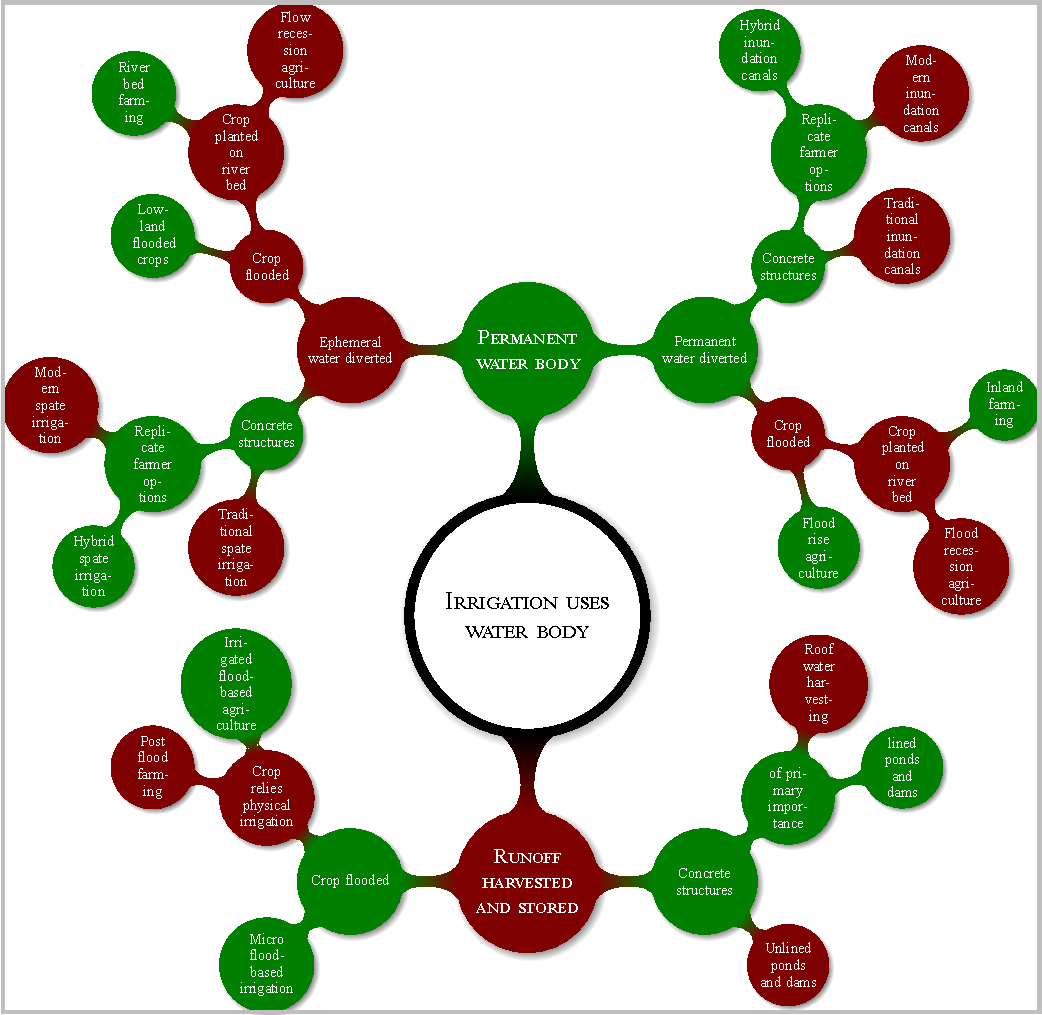
\includegraphics[width=1\linewidth,]{figures/conceptual-class-1} 

}

\caption{A Conceptual classification of flood-based agriculture using simple decision tree rules based on water, vegetation and management aspects}\label{fig:fig2}
\end{figure}

\begin{figure}[!h]

{\centering 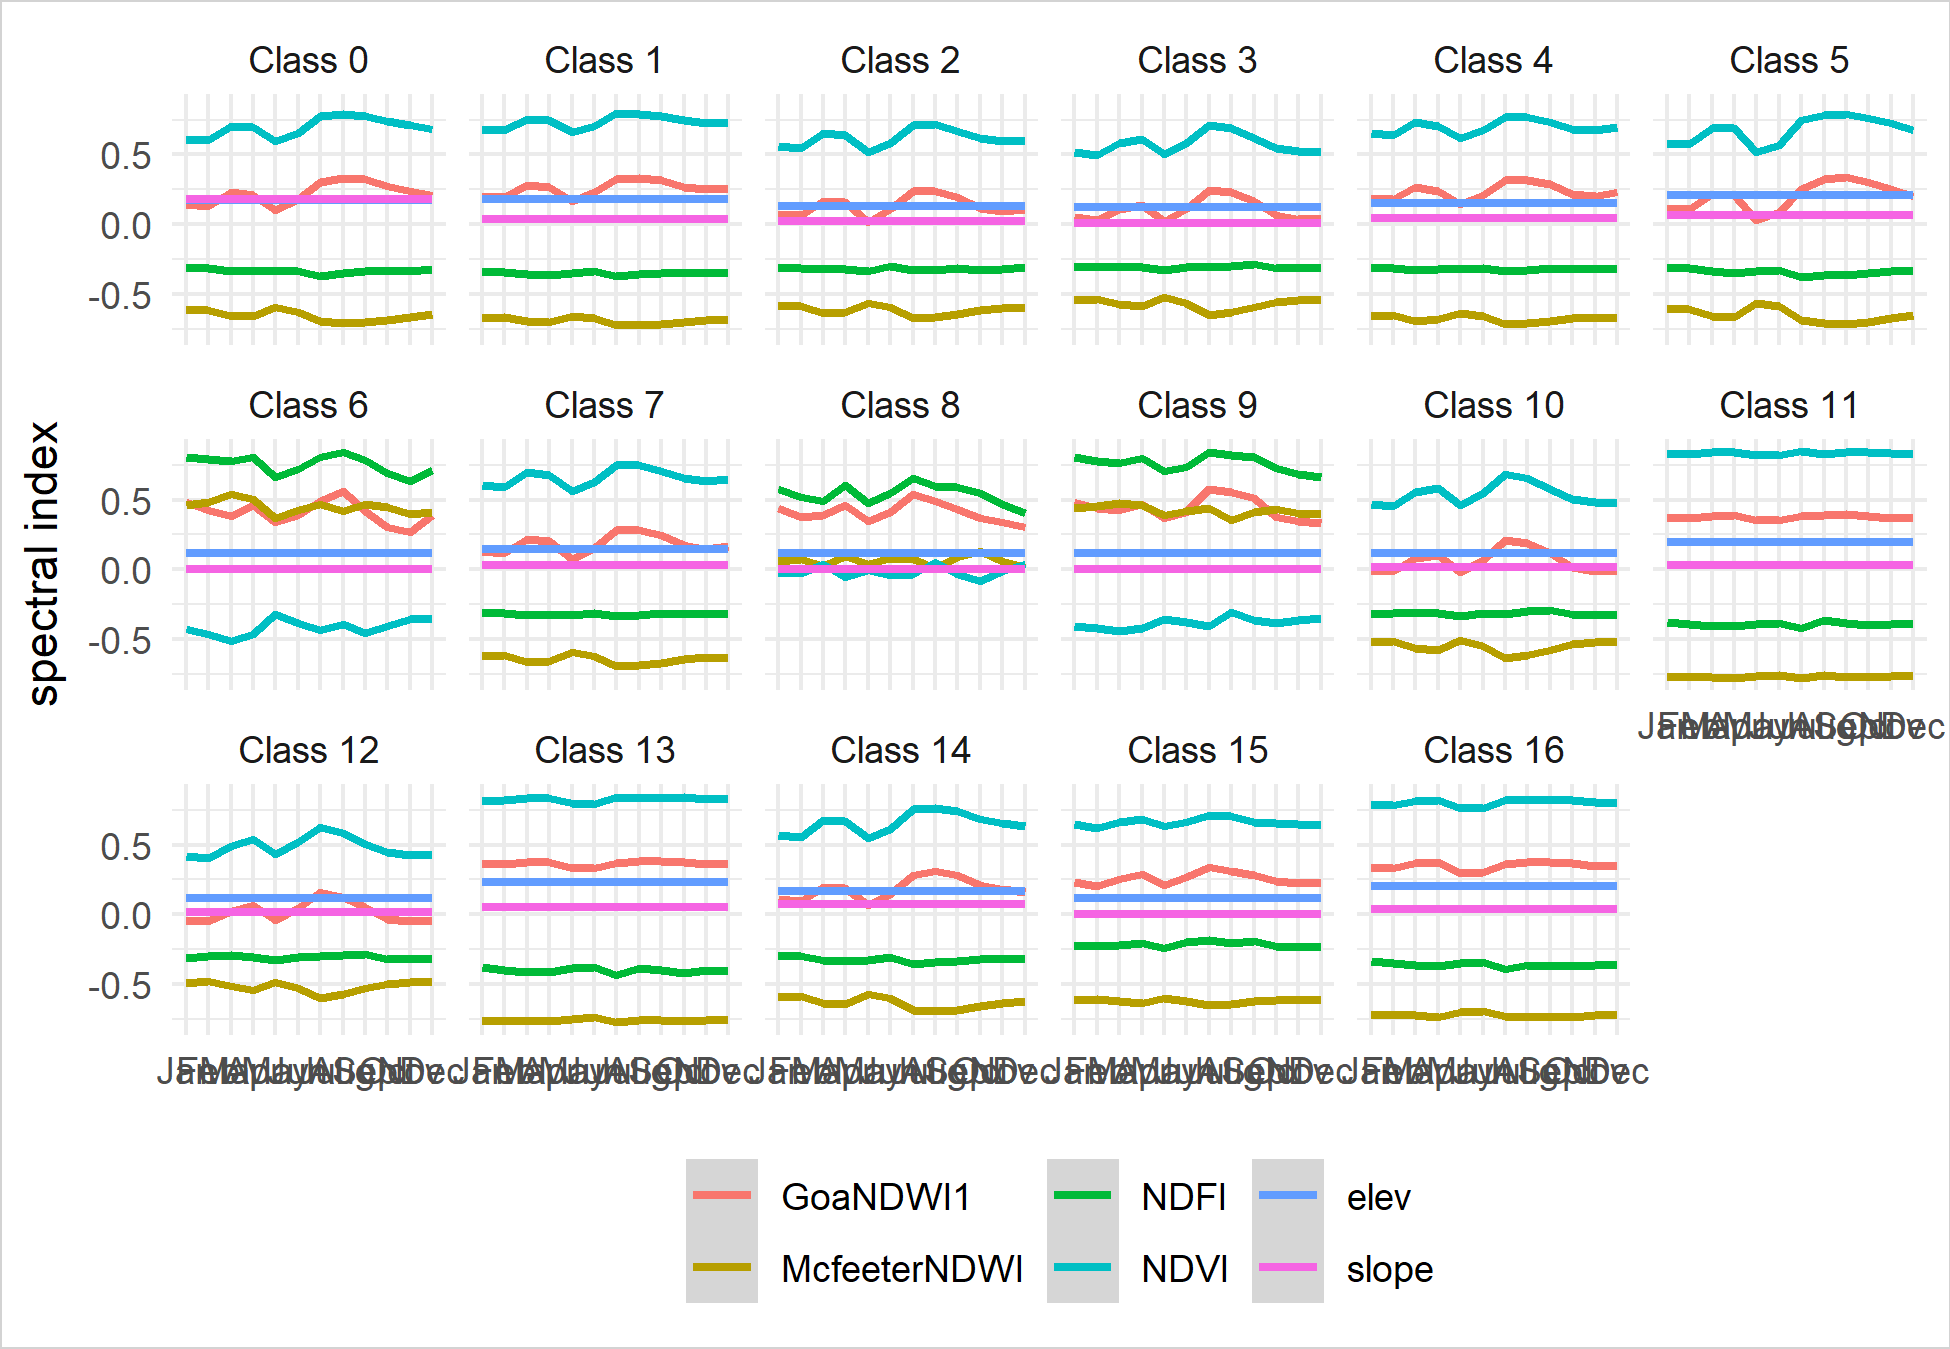
\includegraphics[width=1\linewidth,]{figures/Kisumu_unsuper_NDSI} 

}

\caption{Temporal variability in water and vegetation for different land uses based on an unsupervised classification of 17 classes in Kisumu county, Kenya.}\label{fig:fig4}
\end{figure}

\hypertarget{I}{%
\section{Introduction}\label{I}}

Drylands Agriculture and its transformations have important implications for global food security, particularly under the current population and climate trends (Dixon, Gulliver, \& Gibbon, 2001; FAO, 2017; van Steenbergen, Lawrence, Mehari, Salman, \& Faurès, 2010). Experience has shown that an improvement in farm income results in 2 to 4 times additional non-farm income (Garrity, Dixon, \& Boffa, 2012). Consequently, problems with regards to farm level productivity may produce the opposite effect and may affect food systems on much larger scale. In Eretria, for instance, a country where agriculture play a vital role, the total population would double between 2005 and 2015 causing a food gap of 850, 000 tons (Haile, 2010). Under such impeding constraints, drylands Agriculture is experiencing important transformations to accommodate to these global changes using innovative practices at various scales (FAO, 2017). In flood-based Agriculture, these are shaped by complex social and institutional processes - mainly in forms of soil and water conservation - to produce food under uncertainty (Haile, 2010; Harlan \& Pasquereau, 1969; Puertas, Steenbergen, Haile, Kool, \& Embaye, 2011; van Steenbergen et al., 2010). Despite their extensive and risky nature, flood-based farming systems (FBFS) make substantial contribution to food systems in many drylands areas where they support the livelihoods of millions. For example, it has been estimated that the development of 391,000 ha through spate irrigation would resolve the Eritrean food gap (Haile, 2010). FBFS satisfy the 5 requirements of the 20 major world farming systems for households strategies to escape from poverty and hunger described in Dixon et al.~(2001). These include the agricultural intensification which is achieved through improved production by the means of better water and nutrient supply; the diversification of activities which is conveyed by the ranges of crops grown, the integration of livestock and other off-farms income generating activities; the farm size expansion which is apparent via the encroachment of non-farmed floodplains; the possibility for non-farm income through the investment of farm income into non-farm commercial activities; and the exit or departure from agriculture via migration when the payoff is relatively low.

The promises above-mentioned can be expected considering the value of additional irrigation in rainfed agriculture (Haile, 2010; van Steenbergen et al., 2010) and the willingness of many countries to endorse rural development reforms with specific expectations (FBLN, 2018). Some of these expectations are as ambitious as doubling the country wide production through larger scales flood-based water diversion (Droy \& Morand, 2015; Haile, 2010; van Steenbergen et al., 2010). Meeting such objectives may requires the recognition of the typology of site-specific innovations along with the attuned social processes required for sustainable production. Surprisingly, this recognition is still at the early days because FBFS are missing from the famous farming systems handbooks (Dixon et al., 2001; Garrity et al., 2012; McConnell \& Dillon, 1997). Puertas et al.~(2011) introduce a classification for flood-based farming systems based on the nature and use of the flood inundation. In their guidelines on spate irrigation, van Steenbergen et al.~(2010) provide a classification of spate irrigation, a variant of flood-based agriculture, using on the size of the scheme and management arrangements as the main criteria. In our opinion, however, these classifications lack enough details for operationalizing the basic concepts into a framework for action.

The lack of framing FBFS as standalone topic may have led to the lack of attention of agricultural research and policy to FBFS (Erkossa, Langan, \& Hagos, 2014) and reflected in the common practice to classify agro-ecosystems as either rain-fed or irrigated (Dixon et al., 2001; Garrity et al., 2012; van Steenbergen et al., 2010). However, the peculiar settings under which FBFS are practiced makes them nor rainfed nor irrigated inasmuch as they are rainfed agricultural systems often receiving appreciable amount of irrigation (Haile, 2010; van Steenbergen et al., 2010). Recognising the typology of FBFS would leverage agricultural intensification particularly when site-specific differences are accounted for. Furthermore, even though farmers have unique realities, many share common problems that may transcend any boundary set by mankind (Dixon et al., 2001). In this regards, a classification framework should be anchored at farm level to ultimately categorize similar farmlands into baskets to which similar research and actions would be applied (Dixon et al., 2001; Garrity et al., 2012). Indeed, this would clarify similar investment opportunities, benefit their risk assessment, and cleanly address site-specific problems for optimized agricultural production (Garrity et al., 2012). Prescribing such risk assessment, preferably in quantitative forms, is currently needed because, in most FBFS, decision makers face the challenge of identifying which course of action would result in the greatest agricultural productivity. In many cases, new potentially promising area over which to explore new investment opportunities comport high production risk and uncertainty causing donors and farmers to often remain cautious to invest (Garrity et al., 2012). These promising areas are not often well known or requires the identification of break-through improvements (Droy \& Morand, 2015; Luedeling et al., 2015; van Steenbergen et al., 2010; Whitney, Lanzanova, et al., 2018; Whitney, Shepherd, \& Luedeling, 2018) supporting the need to formally recognize the topic of flood-based agriculture and its variants as standalone thematic area.

Typically farming systems are classified in terms similar natural endowments, entrepreneurship, constraints and opportunities, and development opportunities (Dixon et al., 2001). Identifying the existing FBFS categories may require, in the first place, the identification of key factors determining type-specific hydrology which are shaped by the social mechanisms in place. The objective of this paper is to develop a conceptual framework for system analysis for flood-based agriculture. we start by defining the concepts, reports their importance using publicly available data and other sources, and discusses their typology. We further argue on their potentials and their risky and uncertain nature and propose the use of decision analysis principals to support development interventions.

\hypertarget{VI}{%
\section{reference}\label{VI}}


\end{document}


